\section{Математическая модель динамики судна на нерегулярном волнении}
\label{math_ship}

Для построения модели распределения сил и моментов, действующих на судно, морской объект рассматривается как твердое тело. Введем параметры, описывающие положение корабля в пространстве. Для этого необходимо выбрать локальную систему координат. За начало системы локальных координат примем центр тяжести корабля, а оси расположим так, чтобы ось $x$ была направлена вдоль корабля в направлении носовой части, ось $y$ – влево, ось $z$ – вверх, см. рис. ~\ref{boat_axis}.

\begin{figure}[ht]
\begin{center}
\includegraphics[width=110mm]{boat_axis}
\end{center}
\caption{Локальная система координат и углы вращения судна}
\label{boat_axis}
\end{figure}

Положение судна в пространстве однозначно определяется кортежем из вектора положения центра тяжести и вектора вращения: 
$P=(\mathbf{p},\mathbf{q})$, 
где  
$q=\alpha \mathbf{i}+\beta \mathbf{j}+\gamma \mathbf{k}$, 
где, в свою очередь $\alpha$, $\beta$, $\gamma$,  - углы крена, дифферента и курса, соответственно, а $\mathbf{i}$, $\mathbf{j}$, $\mathbf{k}$ – орты глобальной системы координат. Выпишем второй закон Ньютона:

\begin{equation}
	m \ddot{\mathbf{p}} = \mathbf{F}
	\label{ma=F}
\end{equation}

\begin{equation}
	\mathbf{J}  \ddot{\mathbf{p}} = \mathbf{M}
	\label{jq=M}
\end{equation}

где $m$ – масса корабля и присоединенной жидкости, $\mathbf{J}$ – тензор инерции судна и присоединенной жидкости. Рассмотрим подробнее силу и момент, стоящие в правых частях уравнений \eqref{ma=F} и \eqref{jq=M}. 

Так как ненулевой момент является результатом приложения нецентральной силы, то достаточно рассмотреть следующие силы, действующие на корабль (см. рис. \ref{boat_forces}):
\begin{enumerate}
\item	Сила тяжести, приложенная к центру тяжести и направленная вниз.
\item	Силы давления воды, приложенные к каждой точке корпуса, находящейся в воде, и направленные вдоль нормали к поверхности.
\item	Демпфирующие силы, приложенные к каждой точке корпуса, находящейся в воде, и действующие в направлении против направления движения  данной точки корпуса.
\end{enumerate}

\begin{figure}[ht]
\begin{center}
\includegraphics[width=110mm]{boat_forces}
\end{center}
\caption{Силы, действующие на судно}
\label{boat_forces}
\end{figure}

Суммарные сила и момент, действующие на корабль, могут быть выражены следующим образом:

\begin{equation}
	\mathbf{F} = 
		-\left[ \iint\limits_{S} p \mathbf{n} dS ) 		\right]_{pressure}
		-\left[ \iint\limits_{S} \boldsymbol{\eta} dS ) 	\right]_{damping}
		+ \mathbf{D}
	\label{F=integral}
\end{equation}

\begin{equation}
	\mathbf{M} = 
	-\left[ \iint\limits_{S} 
		\left( p \mathbf{n} \right) \times 
		\left( \mathbf{r} - \mathbf{p} \right) dS	
	\right]_{pressure}
	-\left[ \iint\limits_{S} 
		\left( \boldsymbol{\eta} \right) \times 
		\left( \mathbf{r} - \mathbf{p} \right) dS	
	\right]_{damping}
	\label{M=integral}
\end{equation}

где $S$ --– погруженная поверхность корпуса судна, $D$ --– водоизмещение судна, $p$ –-- давление воды в точке, $\mathbf{n}$ –-- нормаль к поверхности, $r$ --– радиус-вектор точки поверхности в глобальных координатах, $\mathbf{p}$ –-- положение судна в пространстве, $\boldsymbol{\eta}$ --- удельная демпфирующая сила, действующая на единицу поверхности корпуса.

Аналитическое вычисление выражений \eqref{F=integral} и \eqref{M=integral} возможно только для модельной формы корпуса. Как следствие, необходимо на каждом шаге выполнять численное интегрирование. Поверхность корпуса судна разбивается на $N$ малых элементов (размер которых настолько мал, что изменением давления или демпфирующей силы вдоль элемента можно пренебречь), и общая сила и момент рассматривается как сумма сил приложенных к каждому элементу. Таким образом, выражения \eqref{F=integral} и \eqref{M=integral} можно переписать следующим образом:

% Суммирование сил:
\begin{equation}
	\mathbf{F} = 
		-\sum_{i=1}^{N} \left[
			\sigma (\mathbf{r}_i) p_i \mathbf{n}_i \Delta S_i
		\right]
		-\sum_{i=1}^{N} \left[
			\sigma (\mathbf{r}_i) \boldsymbol{\eta}_i \Delta S_i
		\right]
\end{equation}

% Суммирование моментов:
\begin{equation}
	\mathbf{M} = 
		-\sum_{i=1}^{N} \left[
			\sigma (\mathbf{r}_i) p_i \mathbf{n}_i \Delta S_i \times (\mathbf{r_i} - \mathbf{p})
		\right]
		-\sum_{i=1}^{N} \left[
			\sigma (\mathbf{r}_i) \boldsymbol{\eta}_i \Delta S_i \times (\mathbf{r_i} - \mathbf{p})
		\right]
\end{equation}

где:

\begin{equation}
  \sigma(n) = \left\{
  \begin{array}{l l}
    1 & r_z		< 		\Delta z (t, r_x, r_y, 0) \\
    0 & r_z		\geq 	\Delta z (t, r_x, r_y, 0) \\
  \end{array} \right.
\end{equation}

Площадь элемента вычисляется:
\begin{equation}
	\Delta S_i = \frac{S}{N}
\end{equation}

а давление на элемент:
\begin{equation}
	p_i = p(t, r_x, r_y, r_z)
\end{equation}

Расчет силы демпфирования в общем случае является чрезвычайно трудоемким, однако в силу того, что в большинстве штатных и экстремальных режимов эксплуатации судов водоизмещающего типа гидродинамические силы, которыми обусловлены силы демпфирования, вносят лишь не более одну десятой всех сил, действующих на корабль.
Для приближенного определения гидродинамического давления на элемент погруженной поверхности судна можно воспользоваться формулой гидродинамического сопротивления Ньютона \citep{newton}:

\begin{equation}
	p = \rho V^2 \sin ^2 \alpha
\end{equation}

где $V$ --- скорость набегающего потока, $\alpha$ --- угол между поверхностью и набегающим потоком. 
Таким образом, удельная сила действующая на единицу площади может быть выражена как:

\begin{equation}
	\boldsymbol{\eta} = 
		c_x
		\rho 
		\abs{\mathbf{V}}^2 
		\left[  1 - (\norm{\mathbf{V}}, \mathbf{n})  \right]^2
\end{equation}
где $c_x$ --- поправочный к формуле Ньютона коэффициент, задаваемый извне или определяемый экспериментально.

Использование регулярной сетки разбиения корпуса на элементы нецелесообразно, т.к. малые перемещения корабля, могут привести к тому, что целый ряд узлов сетки одновременно погрузится в воду. Как следствие, незначительное изменение осадки или крена может привести к значительному возрастанию гидростатических сил, см. рис. \ref{regular_grid}.

\begin{figure}[ht]
\begin{center}
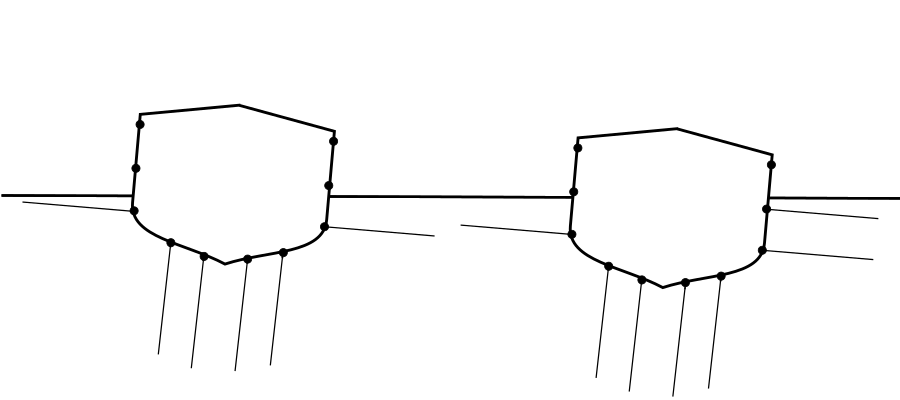
\includegraphics[width=110mm]{regular_grid}
\end{center}
\caption{Иллюстрация вычислительных артефактов за счет скачкообразного изменения гидродинамических сил при использовании регулярных сеток}
\label{regular_grid}
\end{figure}

Для устранения эффектов, указанных на \ref{regular_grid}, для интегрирования \eqref{F=integral} и \eqref{M=integral} используются квадратурные формулы типа Маркова с локально распределенными случайными узлами. Использование статичной или регулярной случайной сетки приводит к появлению нескомпенсированных сил, и, как следствие, самопроизвольному перемещению моделируемого судна. Для избавления от этого эффекта случайная сетка перестраивается на каждом шаге имитационного моделирования. Пример случайной сетки приведен на рис. \ref{monte_carlo}.

\begin{figure}[ht]
\begin{center}
\includegraphics[width=110mm]{monte_carlo}
\end{center}
\caption{Пример сетки с локально-распределенными случайными узлами}
\label{monte_carlo}
\end{figure}

